\chapter{Projektdurchführung}
In diesem Abschnitt der Arbeit wird die eigentliche Durchführung des Projektes näher beschrieben. Dabei wurde das ganze Projekt prototypisch entwickelt, um für spätere Entwicklungen Grundlagen und Wissensstand zu sammeln. Das System soll als Lehrobjekt in verschiedenen Bildungseinrichtungen vermarktet werden. Die Technologien sind im heutigen Zeitalter präsenter denn je, Kinder wachsen mit smarten Innovationen auf. So sollten die zukünftigen Generationen diese Technologien als Bildungsinhalt vermittelt bekommen. Das System in dieser Arbeit soll durch einen mobilen Roboter verschiedene Kompetenzen vermitteln, dazu zählen Programmierung oder logisches Denken. Das System soll eine Basis Applikation auf dem Roboter implementieren und durch verschiedene Mensch-Maschinen-Interfaces sollen unterschiedliche Fähigkeiten vermittelt und dargestellt werden.\cite{RoboterInDerBildung.2021}
% \section{????Material und Methodik}
\section{Anforderungen}
Um ein System zu entwickeln, ist es wichtig, die Anforderung an das System klar zu definieren. Denn erst wenn alle Beteiligten des Systems die Funktionalitäten und Qualitäten bestimmen, kann die Entwicklung beginnen. So können SOLL- und IST-Zustände abgeglichen und gemessen werden, um später bei der Entwicklung und Herstellung des Systems Fehlinterpretation und im allgemeinen Zeitaufwand zu vermeiden. In den folgenden Kapiteln werden die Anforderungen und die beteiligten Personen des Systems dieser Arbeit aufgezeigt.\cite[S.5 ff]{Anforderungsmanagemet.2014}
% \subsection{Anforderungsanalyse}
\subsection{Ermittlung der Stakeholder}
Stakeholder sind Personen oder Personengruppen, die das System durch ihre Anforderungen definieren. \cite[S.18 f]{Anforderungsmanagemet.2014} Die Stakeholder des Systems dieser Arbeit wurden intern bei der Firma Hüttinger durch verschiedene Personen bestimmt, da das System eine Lösung bieten soll, die erst später vermarket werden soll. Dazu haben sich Personen aus der Projektleitung, Softwareentwicklung, Vertrieb und Geschäftsführung zusammengesetzt. Im Folgenden werden die Stakeholdergruppen näher erläutert. \\\\
Die \textbf{Benutzer*in} sind in diesem System Kinder, Schüler*in oder Studierende in Bildungseinrichtungen. Dazu möchten die Benutzer*in ein Programm erstellen, das nicht nur textuell oder bildlich ist, sondern auch die Aktion sehen, die durch das Coden entstanden ist. Überwiegend werden die Benutzer*in aus den MINT-Fächern mit dem System konfrontiert sein. Dabei soll die Fähigkeit zum Programmieren erlernt werden und nicht nur Syntax von Sprachen gelehrt werden.  
\\\\
Die \textbf{Kunden} sind Bildungseinrichtungen wie Schulen, Hochschulen, Universitäten, Museen und Institutionen die Bildung vermitteln aber auch Besucherzentren. Die Kostenträger für das System sind bei Bildungseinrichtungen aber auch oft Kommunen, Städte, Regierungsbezirke oder Staaten.

\subsection{Funktionale Anforderungen}
Funktionale Anforderungen definieren das System hinsichtlich Funktionalität und Verhalten \cite[S.37]{Anforderungsmanagemet.2014}. Im Folgenden werden die funktionalen Anforderungen tabellarisch dargestellt.  
\begin{table}[H]
    % \centering
\begin{tabularx}{\linewidth}{|l|X|}
\hline
\rowcolor{lightgray}
\textbf{Anforderungs-ID} & \textbf{Anforderung}                                                                   \\ \hline
F1              & Der Roboter muss Hindernisse erkennen.                                        \\ \hline
F2              & Der Roboter soll eine Ladestation haben.                                      \\ \hline
F3              & Der Roboter soll Abstandsmessungen mit einem LIDAR (ToF) durchführen.         \\ \hline
F4              & Der Roboter soll mit einer Kamera die unterschiedlichen Hindernisse erkennen. \\ \hline
F5              & Der Roboter soll die Livekamerabilder Streamen.                               \\ \hline
F6              & Der Roboter soll spezielle Grafiken erkennen.                                 \\ \hline
F7              & Der Roboter soll über Lautsprecher dem User Feedback geben.                   \\ \hline
F8              & Der Roboter soll 2D Karten des Labyrinths erstellen.                          \\ \hline
F9              & Der Roboter muss ein Ein/AUS Taster haben.                                    \\ \hline
F10             & Der Roboter soll eine Einheitliche Komponente sein.                           \\ \hline
F11             & Das System soll Fernwartung ermöglichen.                                      \\ \hline
F12             & Das System muss ein offenes Kommunikationsprotokoll haben.                    \\ \hline
\end{tabularx}
    \caption{Funktionale Anforderungen }
    \label{tab:funktionaleAnforderungen}
\end{table}


\subsection{Nicht-funktionale Anforderungen}
Nicht-funktionale Anforderungen erläutern Randbedingungen, die das System haben soll und keine Funktion darstellen \cite[S.37]{Anforderungsmanagemet.2014}. In der folgenden Tabelle werden die nicht-funktionalen Anforderungen wiedergegeben, die das System dieser Arbeit beschreiben. 
\begin{table}[H]
    % \centering
\begin{tabularx}{\linewidth}{|l|X|}
\hline
\rowcolor{lightgray}
\textbf{Anforderungs-ID} & \textbf{Anforderung}                                                                   \\ \hline
NF1              & Der Roboter soll mit Mecanum Rädern ausgestattet sein.                                         \\ \hline
NF2              & Der Roboter soll so klein wie möglich entwickelt werden.                                      \\ \hline
NF3              & Der Roboter soll einen Batterie Status haben.                        \\ \hline
NF4              & Der Roboter soll eine Batterielaufzeit von mindestens 20 min haben. \\ \hline

\end{tabularx}
    \caption{Nicht-funktionale Anforderungen }
    \label{tab:nichtFunktionaleAnforderungen}
\end{table}

\subsection{Architektur}
Die Architektur eines Systems beschreibt die Korrelationen und Wechselwirkung mit einzelnen Komponenten. Die Anforderungen führen dazu, dass die Funktionalitäten definiert werden, die im Anschluss als Systemarchitektur dargestellt werden kann (siehe \autoref{fig:supersystemDekomposition}). Die Entwicklung der Systemarchitektur in dieser Arbeit wurde mithilfe der Software \textit{Papyrus Eclipse} unternommen. Dabei konnte mit der Software \textit{UML} und \textit{SysML} als Modellierungssprache verwendet werden.   

\begin{figure}[H]
 \centering
 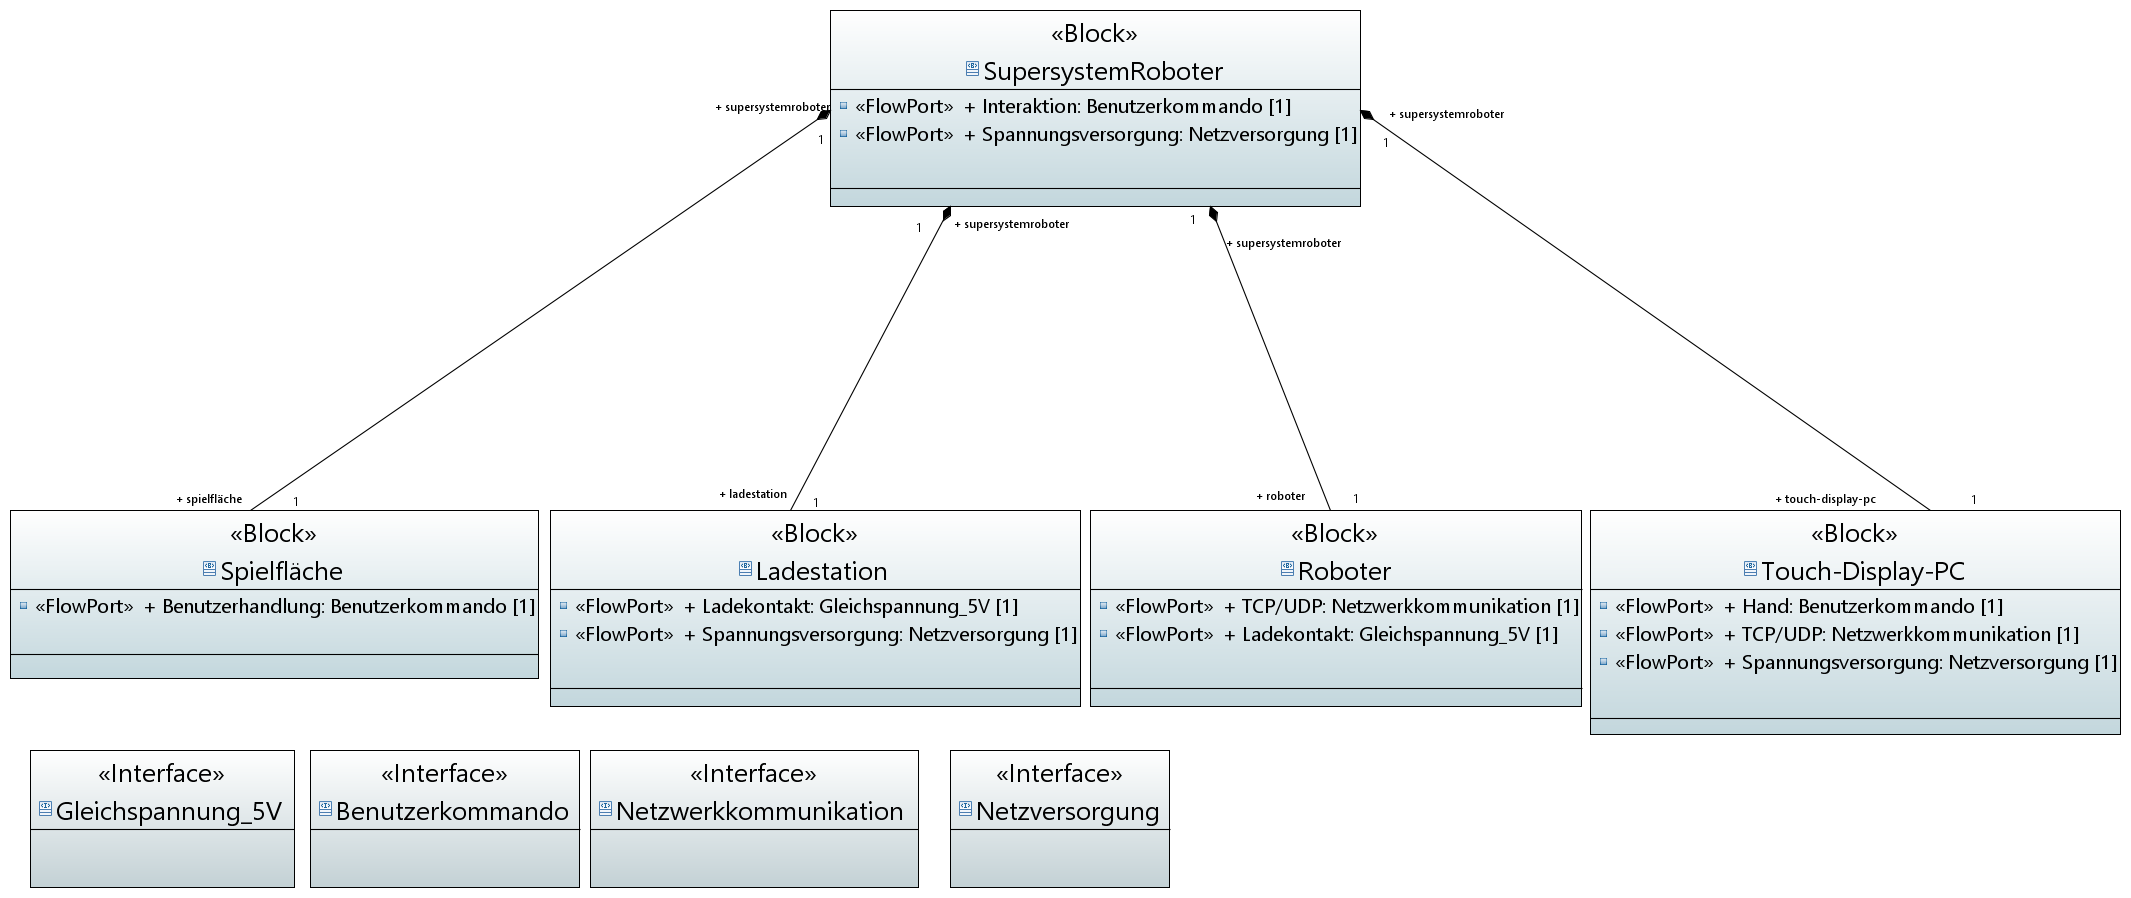
\includegraphics[width=\linewidth]{Bilder/Projektdurchführung/SupersystemDekomposition.PNG}
 \caption{Supersystem Dekomposition dieser Arbeit}
 \label{fig:supersystemDekomposition}
\end{figure}

Das System in dieser Arbeit besitzt mehrere Komponenten, die verbunden sind. Dazu zählen die Benutzer*in, die durch ihre Aktionen und Aktivitäten den mobilen Roboter beeinflussen, dass zu einer Reaktion der Maschine führt. Die Anwender*in können Quellcode über die grafische Oberfläche erstellen oder Anweisungen dem mobilen Roboter übermitteln aber Benutzer*in können als ein Nachbarsystem betrachtet werden. Die ganzen Aktionen der anwendenden Personen werden über die Komponente Touch-Display eingegeben, dadurch ist sie ein Bestandteil des Supersystems. Des Weiteren kann die Spielfläche als ein Stück des Systems erwähnt werden, da sie durch ihre Beschaffenheit die Bewegungsmöglichkeit des Roboters bestimmt. Das elementarste Teil des Systems ist der mobile Roboter, denn erst durch dieses Element können alle Teile des Systems interagieren. Die mobilen Roboter besitzen durch einen Akku eine Lebenszeit, die durch eine Ladestation verlängert werden kann, somit ist die Ladestation auch ein Bestandteil des ganzen Supersystems (siehe \autoref{fig:supersystemKomposition}). 

% Bild vom SuperSystem
\begin{figure}[H]
 \centering
 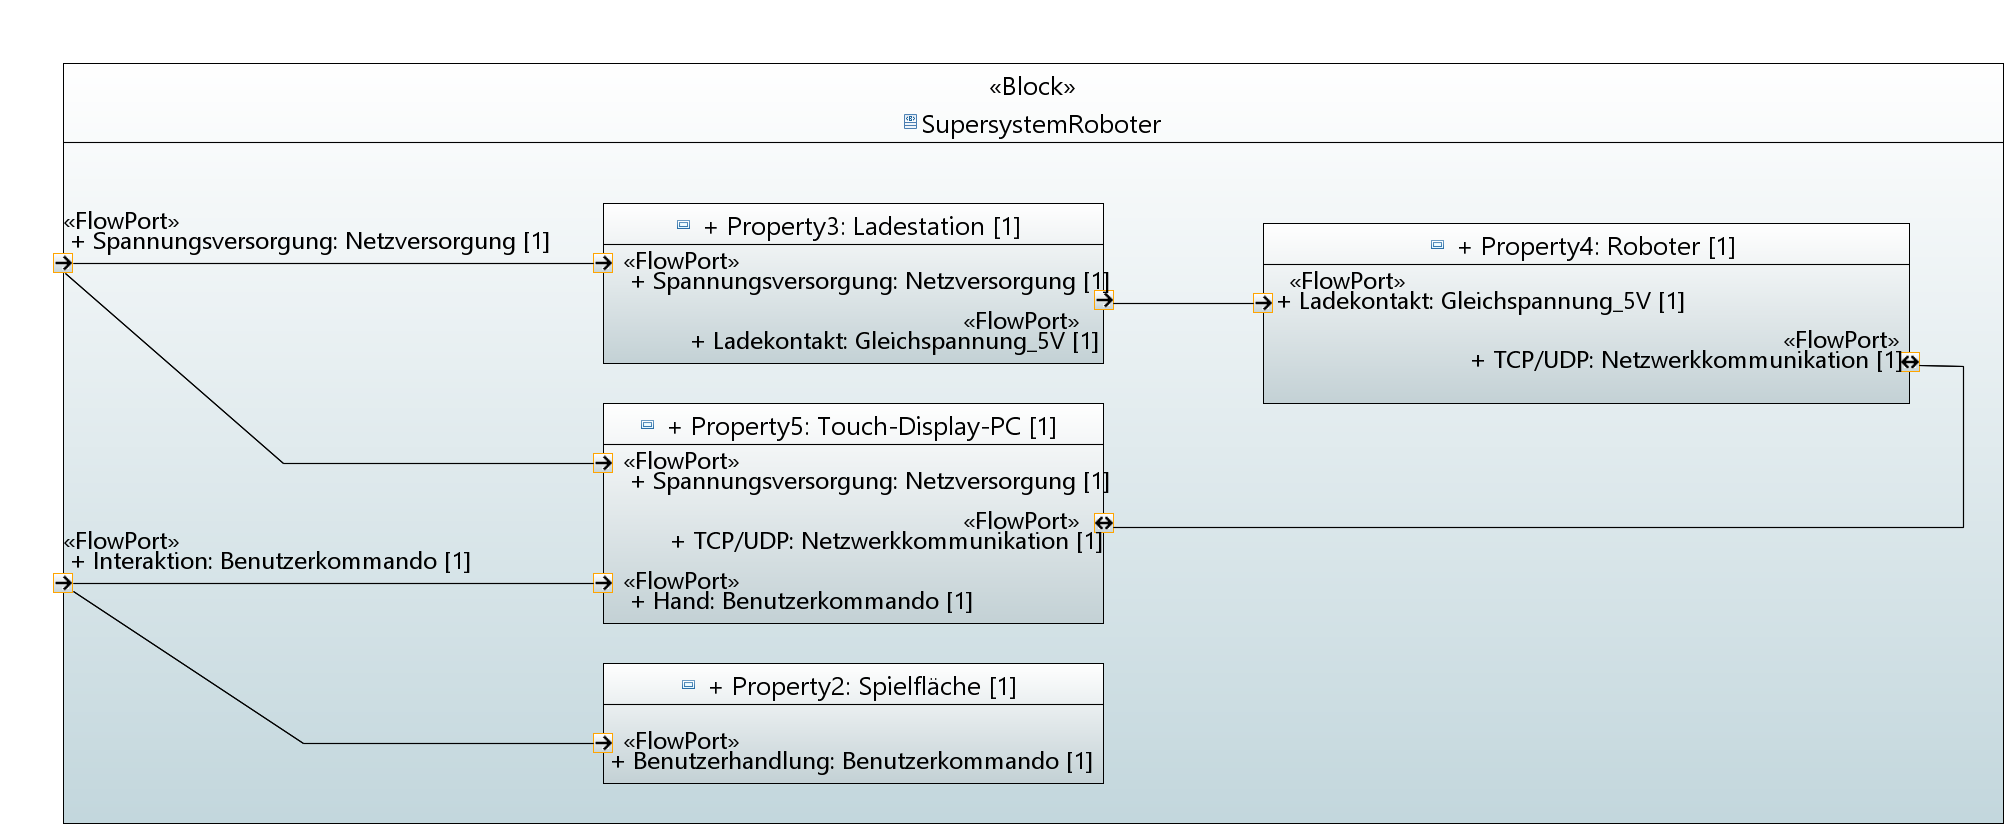
\includegraphics[width=\linewidth]{Bilder/Projektdurchführung/SupersystemKomposition.PNG}
 \caption{Supersystem Komposition dieser Arbeit}
 \label{fig:supersystemKomposition}
\end{figure}


Die separaten Supersystemkomponenten sind wiederum Subsysteme, die auch als Systemarchitektur dargestellt werden können. Im weiteren Verlauf dieses Kapitels wird aber nur die Hauptkomponente der mobile Roboter atomarer dargestellt, da es der Hauptbestandteil dieser Arbeit ist (siehe \autoref{fig:robotersystemKomposition}). 
% Bild System
\begin{figure}[H]
 \centering
 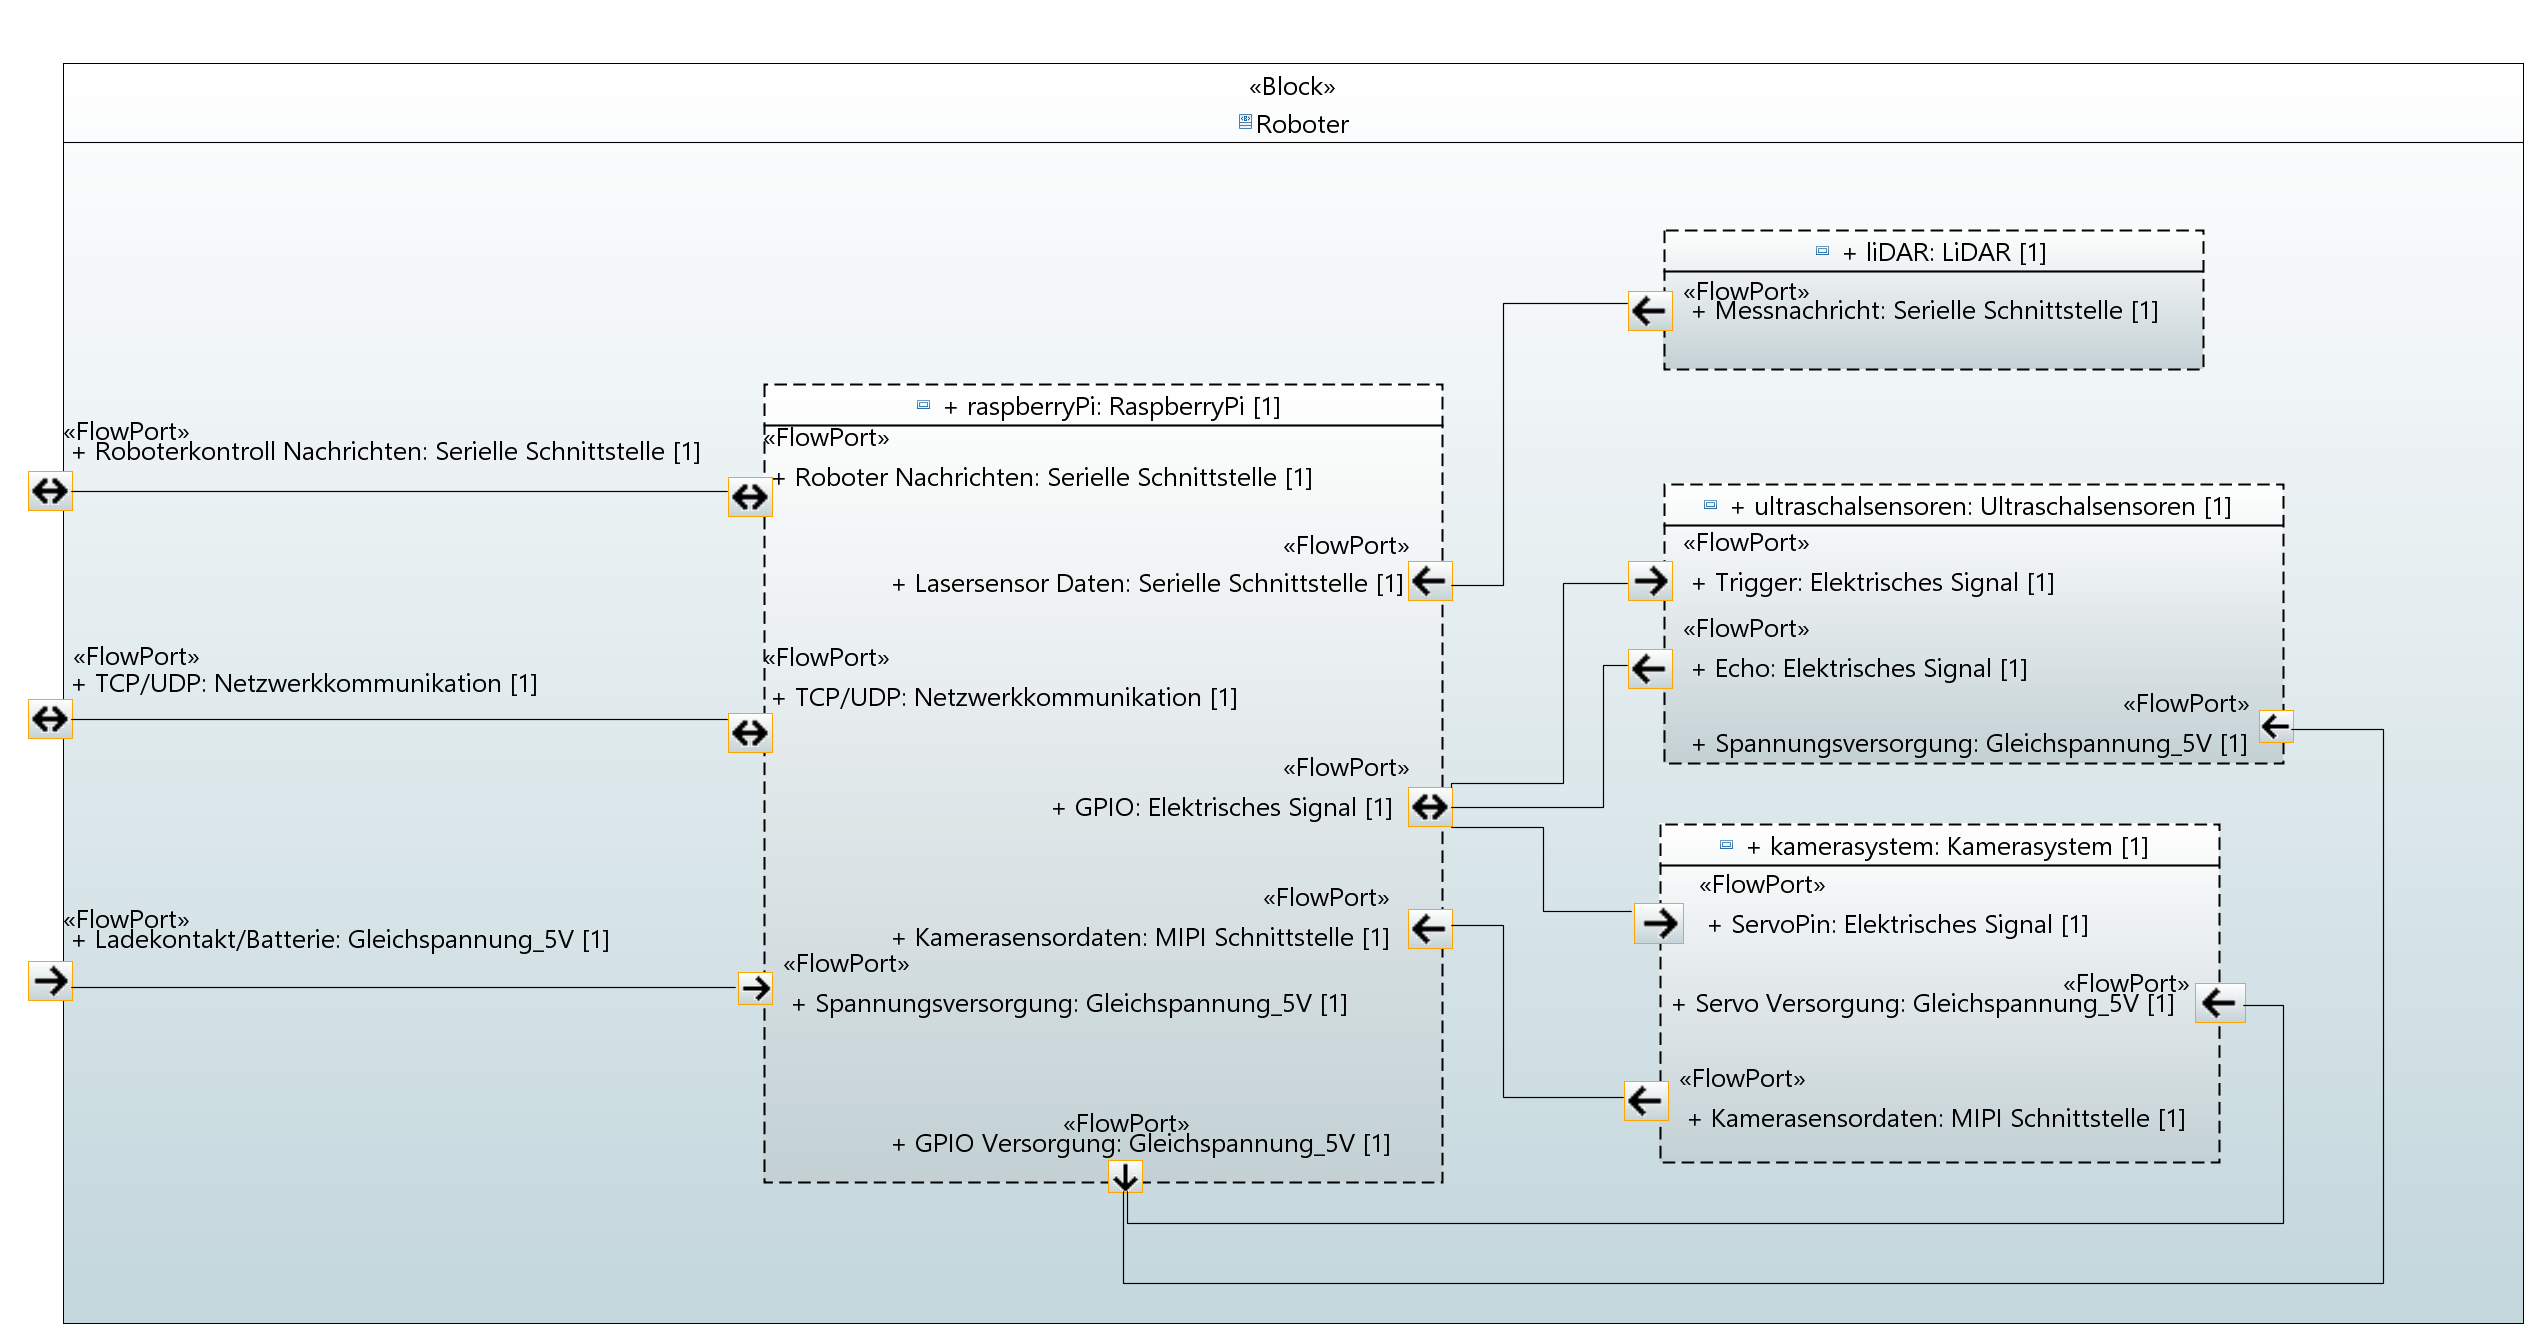
\includegraphics[width=\linewidth]{Bilder/Projektdurchführung/RoboterKomposition.PNG}
 \caption{Mobiler Roboter System Komposition}
 \label{fig:robotersystemKomposition}
\end{figure}

Das System des mobilen Roboters besteht aus Sensoren, Aktoren und einem Rechner. Diese Oberbegriffe repräsentieren eigene System mit Hardware- und Softwarekomponenten.  

% weitere ausführung System mit bilder

\section{Entwurf und Implementierung}
Die Arbeit befasst sich hauptsächlich mit der Programmierung und einer Analyse der Umsetzungsmöglichkeit. Die Systemarchitektur wurde im vorherigen Kapitel umfangreich dargestellt und in diesem Abschnitt wird es um die Implementierung und den Entwurf der Softwarekomponenten gehen. Dabei wurde eine Software entwickelt, die nicht vollständig ist, da es hauptsächlich um die Machbarkeit und einen prototypischen Aufbau ging. Bevor die Softwareimplementierung und der Entwurf näher erläutert wird, werden einige Punkte erwähnt, die für die Umsetzung beschlossen wurden.  

Der mobile Roboter, der verwendet wurde, ist der Kobuki Roboter (siehe \autoref{fig:kobuki}). Dabei handelt sich um einen Roboter mit Differenzialantrieb. Der Kobuki wurde vom Labor mobile Robotik der Technischen Hochschule Nürnberg zur Verfügung gestellt. 

%kobuki bild
\begin{figure}[H]
 \centering
 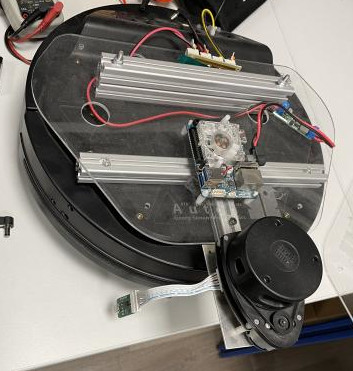
\includegraphics[width=0.4\linewidth]{Bilder/Projektdurchführung/kobuki.jpg}
 \caption{Mobiler Roboter Kobuki}
 \label{fig:kobuki}
\end{figure}

Die ganze Software wurde in der Programmiersprache Python entwickelt. Dabei wurde die Python Version 3.7 verwendet. Die Programmiersprache wurde gewählt da sie mit der Roboterkontrollarchitektur ROS kompatibel ist. Python ist eine Sprache, die auf allen Rechnertypen funktioniert, da es sich um eine interpretierte Sprache handelt und somit nicht direkt mit der Computerhardware arbeitet. Die Programmiersprache ist so entwickelt das sie gut lesbar ist und kompakte Programme erstellt werden können.\cite[S. 12 ff]{PythonKompendium.2021} Es können gut lesbare und kleine Programme entwickelt werden, die auch in der Firma, wo diese Arbeit entstanden ist, leichter interpretiert werden.  

In dieser Arbeit wurde die Roboterkontrollarchitektur ROS verwendet (siehe \autoref{subsubsec:ROS}). Dabei wurde die ROS-Noetic Distribution verwendet. Dabei wird eine Version von ROS-Paketen als ROS-Distribution bezeichnet. Die Pakete haben eine Basis, die verhältnismäßig stabile Software beinhaltet, auf der die Entwicklung zugreift \cite{ROS_Distributions.2021}. Die Distribution wurde gewählt, da ein Kobuki Roboter verwendet wurde. Der Roboter läuft mit der ROS-noetic Version relativ stabil. Es werden ROS-Kobuki-Pakete benutzt, um den Roboter zu bedienen und die Sensoren des Roboters abzufragen. Diesbezüglich werden auch ROS-Pakete verwendet wie \textit{rplidar}. \textit{Rplidar} ist ein Paket für 2D Laserscanner wie ein LiDAR. Sie stellt ROS-Nodes zur Verfügung, um Messwerte vom Sensor zu erhalten.  

\subsection{Implementierung Ultraschall-Sensor}

Der Kobuki der in dieser Arbeit verwendet wurde, ist ein älteres Modell und somit ist auch der LiDAR Scanner eines der ersten Modelle des Herstellers. Die altersbedingten Verschleiße des Scanners haben dazu geführt, dass viele Messpunkte nicht richtig gemessen werden konnten. So gab es kaum seitliche Messwerte vom Roboter. Um einen Pledge-Algorithmus (siehe \autoref{Pledge_Algo}) zu realisieren, braucht es seitliche Messwerte vom Vehikel, damit die Wand verfolgt werden kann. Diesbezüglich wurde die Maschine mit Ultraschall-Sensoren erweitert. Die verwendeten Ultraschall-Sensoren sind HC-SR04, die im Modellbau und Hobby-Embedded Umfeld ihre Anwendung finden.  

Diese Ultraschall-Sensoren wurden am Roboter angebracht und mit dem Raspberry Pi GPIOs verbunden. Die HC-SR04 Sensoren arbeiten mit der Betriebsspannung von $5\; V$. Da die Raspberry Pi Pins mit $3,3\; V$ arbeiten, musste ein Spannungsteiler bestimmt werden, der die Spannung von $5\; V$ auf $3,3\; V$ herabsetzt (siehe \autoref{fig:schaltplanUltraschall}).  

% bild vom Spannungsteiler
\begin{figure}[H]
 \centering
 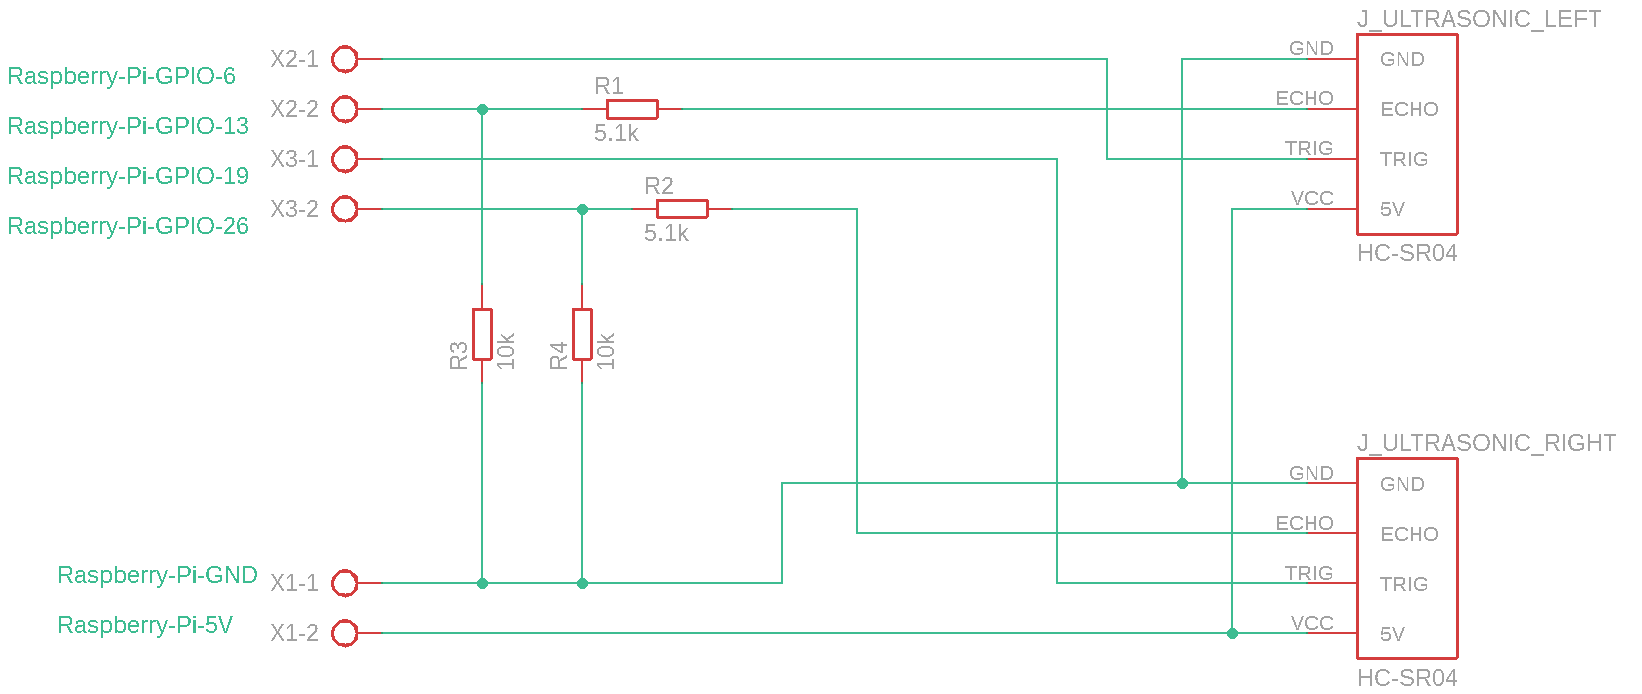
\includegraphics[width=\linewidth]{Bilder/Projektdurchführung/schaltplan.png}
 \caption{Schaltplan mit Spannungsteiler für Ultraschallsensor}
 \label{fig:schaltplanUltraschall}
\end{figure}

% Formel Spannungsteiler 
\begin{align}\label{spannungsteiler}
\centering
\dfrac{U_{Pin}}{U_{Echo}}  &= \dfrac{R_{3}}{R_{1} + R_{3}} \\
\dfrac{U_{Pin}}{U_{Echo}} &= \dfrac{R_{3}}{R_{1} + R_{3}} \; \bigg \vert\; (\;)^{-1} \\
\dfrac{U_{Echo}}{U_{Pin}} &= \dfrac{R_{1} + R_{3}}{R_{3}} = \dfrac{R_{1}}{R_{3}} + \dfrac{R_{3}}{R_{3}} \; \bigg \vert\; - \left(\dfrac{R_{3}}{R_{3}} = 1\right) \\
% \dfrac{U_{Echo}}{U_{Pin}} &= \dfrac{R_{1}}{R_{3}} + \dfrac{R_{3}}{R_{3}} \; \bigg \vert\; - \left(\dfrac{R_{3}}{R_{3}} = 1\right) \\
\dfrac{U_{Echo}}{U_{Pin}} - 1 &= \dfrac{R_{1}}{R_{3}} \;\bigg \vert\; U_{Pin} = 3,3\;V \;\&\; U_{Echo}=5\;V \;\&\; R_{1} = 5,1\; k\Omega \\
R_{3} &= \dfrac{R_{1}}{\dfrac{U_{Echo}}{U_{Pin}} - 1 } = \dfrac{5,1\; k\Omega}{\dfrac{5\; V}{3,3\; V} - 1 } = 9,9\; k\Omega \xLongrightarrow[\text{E24}]{\text{Widerstandsreihe }} R_{3} = 10 k\Omega\\
U_{Pin} &= U_{Echo} \cdot \dfrac{R_{3}}{R_{1} + R_{3}} = 5\; V \cdot \dfrac{10\; k\Omega}{5,1\; k\Omega + 10\; k\Omega} \approx 3,3\; V
\end{align}

Dabei muss nur das Echo Signal vom Sensor mit den Widerständen aus der Formel gesenkt werden (siehe \autoref{spannungsteiler}). Das Trigger Signal kann mit $3,3\; V$ arbeiten da der Low Pegel des Signals bei $< 1\; V$ liegt. Der Spannungsteiler wurde für die Arbeit experimentell auf einer Lochrasterplatine gefertigt.  

Nachdem die Hardware fertiggestellt wurde, konnte die Software für die Sensoren entwickelt werden. Dazu wurde eine Klasse entwickelt, die ein Ultraschall-Sensor ansteuert und das Messergebnis liefert. Die Klasse wurde als Nebenläufigkeit implementiert, damit mehrere Instanzen der Klasse erstellt werden können und nicht geblockt sind (siehe \autoref{fig:activityUltrasonic}). So ist eine zeitgleiche Abfrage der einzelnen Sensoren möglich.   

% Bild Aktivitätsdiagramm Klasse Ultrasonic
\begin{figure}[H]
 \centering
 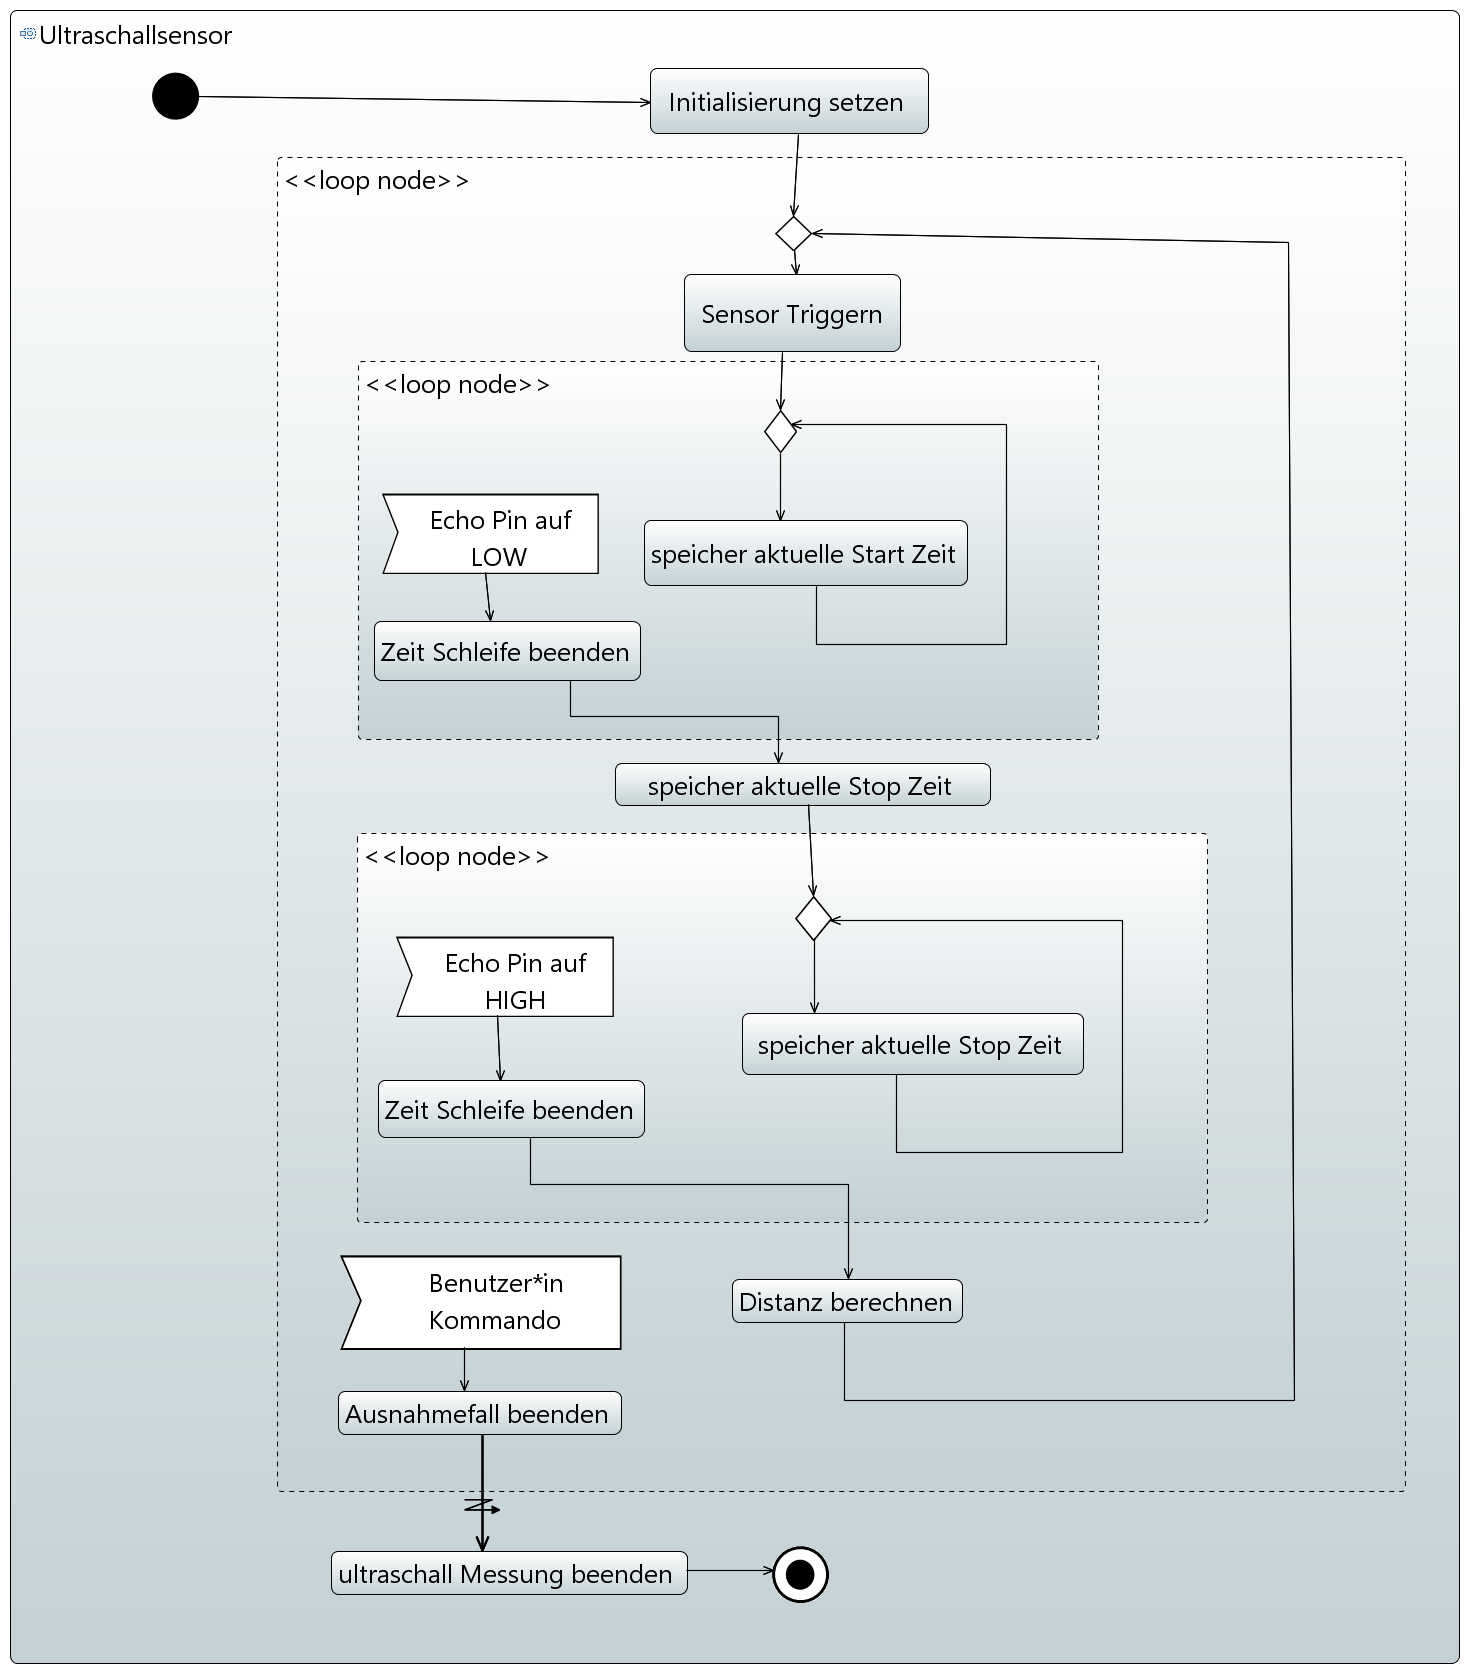
\includegraphics[scale=0.27]{Bilder/Projektdurchführung/UltrasonicActivityDiagram.PNG}
 \caption{Aktivitätsdiagramm des Ultraschallsensors}
 \label{fig:activityUltrasonic}
\end{figure}

Die zwei Ultraschall-Sensoren werden in einer \textit{ultrasonicROS.py} als Instanzen der Klasse erstellt und in einer \textit{while-schleife} mit ROS veröffentlicht. Dazu werden die Messwerte je Sensor über einem Topic veröffentlich. Zudem wurde eine Launch Datei erstellt, um die Sensoren komplett vom System abzukoppeln und als unabhängige Komponenten starten und stoppen zu können.  

\subsection{Implementierung QR-Code Scanner} 

Der Plege-Algorithmus (siehe \autoref{Pledge_Algo}) findet immer einen Ausweg aus einem Labyrinth, wenn ein Ausgang vorhanden ist. Wo es keinen Ausgang gibt, findet der Algorithmus auch keinen und kommt in eine Endlosschleife. Um diese Endlosschleife durchbrechen zu können, wurde eine Raspberry Pi Kamera installiert. Die Firma Kurt Hüttinger GmbH bietet oft Exponate an, die abgeschlossen sind und somit als eine Einheit vermarktet werden. So könnte die Spielfläche des mobilen Roboters geschlossen sein. Damit der Algorithmus auch in diesen Fällen funktioniert, wurde eine Kamera installiert, um mit QR-Codes das Ziel zu markieren. Des Weiteren kann der QR-Code Scanner auch andere Aufgaben übernehmen wie Positionsbestimmung mithilfe von Landmarken.  

Da das Ganze experimentell aufgebaut ist, ist die dominante Seite auch Variable, was dazu führt, dass der Kamerawinkel auch Variable sein muss. Dies wurde durch ein Micro Servomotor SG90 9g gelöst. Die Kamera ist auf dem Servo moniert und je nach dominierender Seite kann der Winkel geschwenkt werden. Der Servomotor kann einen Winkel von $0^\circ$ bis $180^\circ$ einnehmen. Der Servomotor ist auch mit dem Raspberry Pi verbunden und wird durch definierte PWM Signale umgestellt. Dazu wurde auch eine Klasse entwickelt, die dann in einem ROS-Knoten untergebracht ist. Im ROS-Knoten wird ein Topic (siehe \autoref{hl:ROS_Berechnungs_Ebene}) abonniert, dies ermöglicht zur Laufzeit den Winkel einzustellen. Um diese Funktionalität auch vom System abzukoppeln, wurde dies auch in einem eigenständigen ROS-Paket mit Launch Datei erstellt.  

Für den QR-Code Scanner wurde das Quelloffene Softwarepaket ZBar verwendet. Das ZBar Softwarepaket hat für die verschiedenen Programmiersprachen eigenständige Lösungen, so auch für Python mit \textit{pyzabr}. Das Paket ermöglicht aus verschiedenen Quellen, wie Video-Streams, Bilddateien und Sensoren, Barcodetypen zu erkennen und zu decodieren. Dazu wendet das Softwaremodul einen Ansatz zum Erkennen und Decodieren, wie die handelsüblichen Strichcode Scanner und führt eine linearen Scann über die Quelle durch. Es wird jeder Pixel der Quelldatei als unabhängige Probe behandelt \cite{zbar.2011}. Der ganze QR-Code Scanner ist, wie die zuvor genannten Module, auch als eigenständige ROS-Nodes mit Launch Datei realisiert, wobei hier der decodierte Code über einen ROS-Topic publiziert wird.  

\subsection{Implementierung Netzwerkkommunikationsmodule} 

Der Fokus dieser Arbeit ist das API. Die Applikationsschnittstelle soll eine Brücke schaffen zwischen der Anwendung und Roboterkontrollarchitektur, um eine einfache Bedienbarkeit des Roboters zu erhalten. Dabei soll die Schnittstelle über Netzwerk kommunizieren. Dazu wurden die Netzwerkprotokolle wie UDP und TCP auserwählt. Diese Protokolle werden über die IP-Adresse und Port adressiert.  

Zu diesem Zweck wurde ein Modul für die Netzwerkkommunikation entwickelt. Das Python Modul ist nebenläufig entwickelt, da auf das Netzwerk Port aktiv gehört werden muss, um auch eine Nachricht erhalten zu können. Die Klasse definiert dazu alle nötigen Einstellungen. Zudem wurde die Klasse Variable hinsichtlich Protokolltyp aufgebaut. Das Netzwerkprotokoll wird über den Konstruktor bestimmt und je nach Art diesbezüglich definiert. So können auch mehrere Verbindungen aufgebaut werden mit verschiedenen Ports und IP-Adressen. 

\subsection{Implementierung Roboter Module}\label{implRoboterModule}

Neben der Schnittstelle ist das Roboter Modul eine wichtige Komponente. Es vereinfacht den Zugriff auf die Funktionalitäten des mobilen Roboters und der Roboterkontrollarchitektur.  

Die Klasse ist als ein Paralleler Prozess implementiert auch genannt Thread, um eine kontinuierliche Verbindung zu der Roboterkontrollarchitektur ROS aufrecht zu erhalten. Dazu können wichtige Eigenschaften in einer Schleife durchgeführt werden, wie zum Beispiel ob der Weg des Roboters frei ist (siehe \autoref{lst:codelibRobotRun}). 

\lstinputlisting[
language=Python,
label=lst:codelibRobotRun,
caption={Roboter Module Run Methode},
captionpos=b,
numbers=left,
frame=single,
% float,
basicstyle=\fontsize{11}{11}\ttfamily,
keywordstyle=\color{blue},
commentstyle=\color{olive},
stringstyle=\color{red},
]{Quellcode/libRobotRun.py}

Dabei kann die Klasse auch als ein Python Modul verwendet werden, um Roboter mithilfe von ROS zu bedienen. So kann sie nicht nur für die Schnittstelle verwendet werden, sondern auch universeller eingesetzt werden. Das Modul ermöglicht auch durch Umrechnungen Einzelschritt Bewegungen. Dies kann genutzt werden, um Pfade vorzuprogrammieren und sie abzuspielen. Die Funktionalitäten des Roboters sind so in einer Klasse ausgelagert und vereinfachen das API.  

\subsection{Implementierung Pledge-Algorithmus}

Es wurde ein eigenständiges Objekt entwickelt für den Pledge-Algorithmus. Dazu wurde die Klasse als ein Zustandsautomat implementiert (siehe \autoref{fig:zustandsautomatPledgeAlgo}). Der Ablauf von Zustandsautomaten ist es, dass Zustände eingenommen werden und nur durch eine Bedingung ein Zustandswechsel stattfindet. So ist ein Zustandsautomat ein geblocktes System. Um aber den Ablauf der API nicht zu gefährden, ist die Klasse parallel ausführbar. So kann jederzeit der Algorithmus beendet und erneut gestartet werden, ohne Auswirkungen auf das API zu haben.  
\begin{figure}[H]
 \centering
 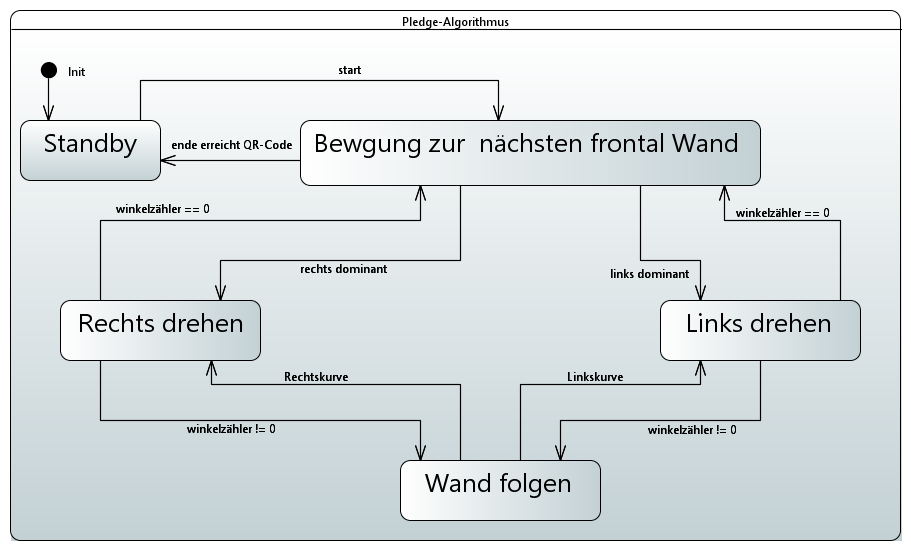
\includegraphics[width=\linewidth]{Bilder/Projektdurchführung/Pledge-Algo-State-machines.PNG}
 \caption{Zustandsautomat Pledge-Algorithmus}
 \label{fig:zustandsautomatPledgeAlgo}
\end{figure}

Die einzelnen Zustände sind eigenständige Methoden. So wird beim Zustand \textit{“Bewegung zur nächsten frontalen Wand”} der mobile Roboter mit einer Vorwärts Geschwindigkeit angesteuert und in der Dauerschleife der Sensorwert vom LiDAR verglichen. Sobald der Wert des Sensors eine bestimmte Schwelle unterschreitet, wird dieser Zustand beendet und zum nächsten Zustand gewechselt (siehe \autoref{lst:codepledgeMoveToNextWall}).\\ 

\lstinputlisting[
language=Python,
label=lst:codepledgeMoveToNextWall,
caption={Klassenmethode vom Zustand "Bewegung zur nächsten frontalen Wand"},
captionpos=b,
numbers=left,
frame=single,
% float,
basicstyle=\fontsize{11}{11}\ttfamily,
keywordstyle=\color{blue},
commentstyle=\color{olive},
stringstyle=\color{red},
]{Quellcode/pledgeMoveToNextWall.py}



Die Zustände Rechts bzw. Links Drehen sind $|90^{\circ}|$ Drehungen. Die werden über das Roboter Modul direkt angesteuert. Dies ist möglich durch die Schrittbewegungsfunktionalität des Moduls, wie bereits erwähnt im \autoref{implRoboterModule}. Zusätzlich zur Drehung wird ein Winkelzähler mitgezählt. Ein weiterer Zustand ist \textit{“Wand folgen”}, dass so ähnlich wie der Zustand \textit{“Bewegung zur nächsten frontalen Wand”} funktioniert. Bei dieser Klassenmethode werden die Ultraschallsensoren verwendet, um den Abstand zur Wand verfolgen zu können.

\subsection{Implementierung API}
Das ganze System wird durch das API verbunden und bindet somit alle Partikel miteinander. Die Schnittstelle selbst ist als ein Spiel-Algorithmus aufgebaut. Dabei werden alle nötigen Instanzen gebildet und im Anschluss wird eine Dauer-Schleife gestartet. Die Spiel-Schleife, auch oft \textit{Game Loop} genannt, hat drei entscheidende Funktionalitäten. Dazu zählt als Erstes der \textit{Input}, also die Benutzereingaben, diese sind in diesem Fall über Netzwerknachrichten abgedeckt. Als zweite Funktion dient das \textit{Update} dazu, Berechnungen durchzuführen oder Positionen zu bestimmen. Die dritte Funktionalität der Schleife ist \textit{Output} oder \textit{Render}, dass für die Ausgabe von neu errechneten Werten fungiert. Diese drei Funktionen werden nicht nur in der Spieleprogrammierung verwendet, sondern auch in vielen verschiedenen Branchen wie in der Automatisierung oder auch allgemein bei Computern. Diese Methoden werden anders genannt, aber eines wird häufiger in diesem Zusammenhang verwendet, das \textit{EVA-Prinzip}. Das \textit{EVA-Prinzip} steht für Eingabe, Verarbeitung und Ausgabe. So wurde auch die Schnittstelle für diese Arbeit aufgebaut (siehe \autoref{lst:codegameLoopl}). Als Eingabe fungieren die Netzwerknachrichten, der Verarbeitungsschritt ist die Verarbeitung der Nachrichten und als Ausgabe werden Roboter Steuerbefehle versendet. Durch diese Methode kann zu jeder Eingabe eine Reaktion folgen.

\lstinputlisting[
language=Python,
label=lst:codegameLoopl,
caption={Game Loop der Schnittstelle},
captionpos=b,
numbers=left,
frame=single,
% float,
basicstyle=\fontsize{11}{11}\ttfamily,
keywordstyle=\color{blue},
commentstyle=\color{olive},
stringstyle=\color{red},
]{Quellcode/engineLoop.py}

 
% Bild API Struktur und vielleicht eine komplette Klassen Übersicht